\documentclass[a4paper]{cas-sc}

\usepackage[numbers]{natbib}
\usepackage[utf8]{inputenc}
\usepackage{enumitem}
\usepackage{lmodern}
\usepackage{graphicx}
\usepackage{amsmath}
\usepackage{amssymb}
\usepackage{microtype}
\usepackage{indentfirst}
\usepackage{float}
\usepackage{placeins}
\usepackage{caption}
\usepackage{booktabs}
\usepackage{algorithm}
\usepackage{algpseudocode}
\usepackage{hyperref}

\setlength{\parindent}{2em}
\setlist[enumerate]{listparindent=\parindent,itemindent=\parindent}
\setlength{\emergencystretch}{2em}

% Author macros
\def\tsc#1{\csdef{#1}{\textsc{\lowercase{#1}}\xspace}}
\tsc{WGM}
\tsc{QE}

\begin{document}
\let\WriteBookmarks\relax
\def\floatpagepagefraction{1}
\def\textpagefraction{.001}

% Short title
\shorttitle{A SAT Solving Approach to the Cyclic Bandwidth Minimization Problem}    
% Short author
\shortauthors{Lê Nam Huy}  
% Main title of the paper
\title [mode = title]{A SAT Solving Approach to the Cyclic Bandwidth Minimization Problem}  
% Author
\author{Student: Lê Nam Huy\\24021516}

\begin{abstract}
The Cyclic Bandwidth Minimization Problem (CBMP) is an NP-hard graph layout problem that seeks an injective assignment of graph vertices to positions arranged on a circle such that the maximum cyclic distance between adjacent vertices is minimized. In this paper, we propose a scalable Boolean Satisfiability (SAT) framework for CBMP. We formulate CBMP through an iterative feasibility search that combines Order Encoding for distance constraints, Commander Encoding for bijective permutation constraints, and dual symmetry-breaking techniques (rotation and reflection) designed to prune the $2N$-fold dihedral symmetry of the cyclic search space. In addition, an initial upper bound is seeded using the Reverse Cuthill--McKee (RCM) heuristic layout. We conduct an exhaustive experimental campaign across 16 benchmark instances derived from power transmission networks, comparing five CDCL SAT solvers (CaDiCaL~195, Glucose~4, MapleChrono, MiniSat~2.2, and Lingeling) against state-of-the-art baselines: Constraint Programming (OR-Tools CP-SAT) and Mixed-Integer Linear Programming (IBM ILOG CPLEX). Our findings show that rotation and reflection symmetry breaking achieve up to a $22.77\times$ speedup on medium boundary instances and reduce median runtime by over $59\%$ across randomized graph families. Furthermore, the best SAT configuration proves global optimality on instances where CP-SAT times out (e.g., \texttt{662\_bus\_n100}), while CPLEX is severely constrained by model size limits.
\end{abstract}

\begin{keywords}
Cyclic Bandwidth Minimization \sep Propositional Satisfiability \sep Order Encoding \sep Commander Encoding \sep Symmetry Breaking \sep Constraint Programming
\end{keywords}

\maketitle

% =========================================================================
\section{Introduction}
% =========================================================================

Graph layout problems seek to embed the vertices of a graph into a host metric space while minimizing a geometric objective defined over the edges \citep{diaz2002survey}. A prominent member of this family is the \textit{Bandwidth Minimization Problem} (BMP), where vertices are assigned to integer positions on a linear line such that the maximum length of any edge is minimized. When the host topology is wrapped into a ring or circle, the problem becomes the \textit{Cyclic Bandwidth Minimization Problem} (CBMP) \citep{leung1984cyclic}.

\subsection{Problem Context and Motivation}
CBMP arises naturally in numerous practical domains:
\begin{enumerate}
    \item \textbf{VLSI Design and Circular Layouts}: In circular integrated circuit design, macrocells and logical modules are arranged in a ring to facilitate routing channels and minimize the maximum interconnect length, which directly impacts capacitive load and propagation delay \citep{kahng2011vlsilayout}.
    \item \textbf{Interconnection Networks and Ring Topologies}: Metropolitan area networks (MANs), optical ring networks (SONET/SDH), and distributed ring-based multicomputer architectures rely on circular vertex embeddings to minimize packet hop counts and prevent communication bottlenecks \citep{leung1984cyclic}.
    \item \textbf{Matrix Bandwidth and Wavefront Reduction}: In scientific computing and finite element analysis, permuting sparse symmetric matrices to reduce their cyclic envelope accelerates iterative linear system solvers and parallel sparse matrix-vector multiplications.
\end{enumerate}

CBMP is known to be NP-hard in the general case, even when restricted to trees with maximum degree 3 or caterpillar graphs \citep{leung1984cyclic, diaz2002survey}. Consequently, exact methods face substantial combinatorial challenges due to the factorial size of the permutation search space ($N!$) and the cyclic distance metric.

\subsection{Research Objective and Proposed Approach}
Existing exact methodologies predominantly rely on branch-and-bound linear integer programming or dedicated constraint programming formulations. However, propositional satisfiability (SAT) solvers have demonstrated remarkable efficiency in combinatorial search due to Conflict-Driven Clause Learning (CDCL), two-literal watching, and learned clause management \citep{biere2021handbook}.

In this work, we design, implement, and rigorously evaluate an exact SAT-based optimization framework for CBMP. We model the problem as a sequence of decision problems, shrinking the candidate cyclic bandwidth bound $\text{UB}$ iteratively until the formula becomes unsatisfiable (UNSAT), thereby establishing global optimality. To ensure scalability, our approach integrates:
\begin{itemize}
    \item A compact CNF encoding combining \textbf{Commander Encoding} for the bijective vertex-to-label cardinality constraints and \textbf{Order Encoding} for cyclic distance bounds, resulting in $\mathcal{O}(|E| \cdot N + N^2)$ clauses.
    \item \textbf{Dual symmetry breaking}: Fixing an anchor vertex at label 0 (rotation symmetry breaking) and ordering the relative placement of two distinct adjacent positions (reflection symmetry breaking), eliminating the $2N$-fold dihedral search space redundancy.
    \item \textbf{Heuristic upper bounding}: Seeding the iterative search with a valid permutation generated by the Reverse Cuthill--McKee (RCM) heuristic \citep{cuthill1969rcm}, reducing the number of costly SAT iterations.
\end{itemize}

\subsection{Summary of Contributions}
The main contributions of this paper are:
\begin{enumerate}
    \item \textbf{Principled SAT Formulation}: A mathematically rigorous and clause-efficient encoding for CBMP combining Commander and Order representations.
    \item \textbf{Symmetry Breaking and Formal Solution Counting}: Correct mathematical formulation of rotation and reflection symmetry breaking, validated by exact solution enumeration on benchmark topologies confirming the theoretical reduction ratios ($N$ and $2$).
    \item \textbf{Extensive Empirical Evaluation}: A reproducible benchmark suite over 16 MatrixMarket graphs comparing 5 CDCL SAT solvers, OR-Tools CP-SAT, and IBM CPLEX across multiple seeds and graph families.
    \item \textbf{Phase and Ablation Analyses}: A granular decomposition showing that the final UNSAT iteration dominates total runtime ($60\%\text{--}90\%$), explaining why symmetry breaking provides decisive speedups (up to $22.77\times$).
\end{enumerate}

% =========================================================================
\section{Background}
% =========================================================================

\subsection{Graph Notation and Cyclic Bandwidth}
Let $G = (V, E)$ be a simple, connected, undirected graph with vertex set $V = \{v_0, v_1, \dots, v_{N-1}\}$ ($|V| = N$) and edge set $E$ ($|E| = M$). Let $\Delta$ denote the maximum vertex degree of $G$.

A \textit{labeling} or \textit{layout} of $G$ is a bijection $f: V \to \{0, 1, \dots, N-1\}$. Under this labeling, the positions $0, 1, \dots, N-1$ are arranged consecutively along a cycle $\mathcal{C}_N$. For any two labels $i, j \in \{0, \dots, N-1\}$, the \textit{cyclic distance} is defined as:
\begin{equation}
    d(i, j) = \min\bigl(|i - j|,\; N - |i - j|\bigr).
    \label{eq:cyclic_distance}
\end{equation}
The cyclic distance satisfies $0 \le d(i, j) \le \lfloor N/2 \rfloor$ for all $i, j$.

The \textit{cyclic bandwidth of $G$ under layout $f$}, denoted $B_c(G, f)$, is the maximum cyclic distance between adjacent vertices:
\begin{equation}
    B_c(G, f) = \max_{(u, v) \in E} d\bigl(f(u), f(v)\bigr).
\end{equation}
The \textit{Cyclic Bandwidth Minimization Problem} (CBMP) asks for a layout $f^*$ that attains the minimum cyclic bandwidth:
\begin{equation}
    B_c(G) = \min_{f} B_c(G, f).
\end{equation}

\subsection{Theoretical Lower Bounds}
A well-known structural lower bound for cyclic bandwidth is derived from the maximum vertex degree $\Delta$. For any vertex $u$ with degree $\operatorname{deg}(u)$, its neighbors must be assigned distinct labels along the cycle. Since the cyclic distance cannot exceed the available positions on either side of $f(u)$, we have:
\begin{equation}
    B_c(G) \ge LB_{\text{degree}} = \left\lceil \frac{\Delta}{2} \right\rceil.
    \label{eq:lb_degree}
\end{equation}
While stronger lower bounds based on graph density or spectral properties exist, $LB_{\text{degree}}$ provides a reliable, immediate baseline against which upper bounds can be checked.

\subsection{SAT and Propositional Logic}
A Boolean variable $x$ takes values in $\{\text{true}, \text{false}\}$. A literal is a variable $x$ or its negation $\neg x$. A clause is a disjunction of literals, and a formula in Conjunctive Normal Form (CNF) is a conjunction of clauses. A SAT solver determines whether a CNF formula is satisfiable (SAT) or unsatisfiable (UNSAT). Modern solvers use Conflict-Driven Clause Learning (CDCL) \citep{biere2021handbook}, which incorporates unit propagation, non-chronological backtracking, conflict clause learning, and dynamic variable selection heuristics (e.g., VSIDS).

Cardinality constraints enforce that at least one (ALO), at most one (AMO), or exactly one (EO) literal in a set $X = \{x_1, \dots, x_n\}$ evaluates to true.

\subsection{Symmetries in Cyclic Embeddings}
For any layout $f: V \to \{0, \dots, N-1\}$, rotating all labels by an offset $c \in \{0, \dots, N-1\}$ via $f_{\text{rot}}(u) = (f(u) + c) \bmod N$ leaves all pairwise cyclic distances $d(f_{\text{rot}}(u), f_{\text{rot}}(v))$ unchanged. Similarly, reflecting all labels across diameter 0 via $f_{\text{ref}}(u) = (N - f(u)) \bmod N$ preserves all cyclic distances. The automorphism group of the cycle $\mathcal{C}_N$ is the dihedral group $D_N$, containing $2N$ isometric symmetries ($N$ rotations and $N$ reflections). Without symmetry breaking, every valid layout belongs to an equivalence class of size up to $2N$, forcing the SAT solver to repeatedly explore symmetric subtrees during search and UNSAT proofs.

% =========================================================================
\section{Method}
% =========================================================================

Our SAT encoding models the decision problem: given a graph $G = (V, E)$ and an integer bound $K \in [1, \lfloor N/2 \rfloor]$, does there exist a layout $f: V \to \{0, \dots, N-1\}$ such that $d(f(u), f(v)) \le K$ for all $(u, v) \in E$?

\subsection{Decision Variables}
We employ two families of Boolean variables:
\begin{enumerate}
    \item \textbf{Direct label variables} $X = \{x_u^i \mid u \in \{0, \dots, N-1\},\; i \in \{0, \dots, N-1\}\}$, where:
    \begin{equation}
        x_u^i = \text{true} \iff f(u) = i.
    \end{equation}
    There are $N^2$ direct variables.
    \item \textbf{Order variables} $G = \{g_u^i \mid u \in \{0, \dots, N-1\},\; i \in \{0, \dots, N\}\}$, where:
    \begin{equation}
        g_u^i = \text{true} \iff f(u) \ge i.
    \end{equation}
    There are $N(N + 1)$ order variables.
\end{enumerate}

\subsection{Bijective Assignment: Commander Encoding}
A valid layout requires that every label $i \in \{0, \dots, N-1\}$ is assigned to exactly one vertex $u \in V$. That is, for each column $i$, the variable set $X^i = \{x_0^i, x_1^i, \dots, x_{N-1}^i\}$ must satisfy $\text{EO}(X^i) = \text{ALO}(X^i) \land \text{AMO}(X^i)$.

Rather than using a quadratic pairwise encoding ($\mathcal{O}(N^2)$ binary clauses per label) or a 2D product encoding, our implementation employs \textbf{Commander Encoding} \citep{klieber2007efficient} with group width $W = 3$ (as implemented in \texttt{alo\_amo\_eo\_encodings.py}).

The algorithm partitions the $N$ variables into $\lceil N/W \rceil$ disjoint groups of size at most 3:
\begin{enumerate}
    \item \textbf{Intra-group AMO}: For each group $\{x_{g,1}, x_{g,2}, x_{g,3}\}$, standard pairwise mutex clauses are added:
    \begin{equation}
        (\neg x_{g,1} \lor \neg x_{g,2}) \land (\neg x_{g,2} \lor \neg x_{g,3}) \land (\neg x_{g,3} \lor \neg x_{g,1}).
    \end{equation}
    \item \textbf{Commander Variables}: For each group $g$, an auxiliary commander variable $c_g$ is introduced to represent whether any variable in group $g$ is true:
    \begin{align}
        x_{g,j} &\implies c_g \iff (\neg x_{g,j} \lor c_g) \quad \forall j, \\
        c_g &\implies \bigvee_{j} x_{g,j} \iff \left(\neg c_g \lor \bigvee_{j} x_{g,j}\right).
    \end{align}
    \item \textbf{Recursive Inter-group AMO}: The commander variables $\{c_1, c_2, \dots\}$ are recursively partitioned until a single top-level group remains.
    \item \textbf{Top-level ALO}: A single ALO clause is posted over the final top-level commander variables:
    \begin{equation}
        \bigvee_{k} c_{\text{top}, k}.
    \end{equation}
    Because the implication $c_g \implies \bigvee_j x_{g,j}$ propagates downwards through all recursion levels, satisfying the top-level ALO guarantees that at least one original variable is true. Together with the hierarchical AMO constraints, this guarantees that exactly one variable in $X^i$ is true.
\end{enumerate}
Commander encoding requires $\mathcal{O}(N)$ auxiliary variables and $\mathcal{O}(N)$ clauses per label, maintaining linear footprint per label without the routing overhead of deep sorting networks.

\subsection{Order Encoding and Linking Clauses}
The ladder variables $g_u^i$ represent the step function $f(u) \ge i$ \citep{tamura2009order}. They are governed by two sets of constraints:

\paragraph{Monotonicity and Boundary Constants:}
For each vertex $u$, the order variables must form a contiguous sequence of true values followed by false values:
\begin{align}
    g_u^0 &= \text{true}, \qquad g_u^N = \text{false}, \label{eq:order_bounds} \\
    g_u^{i+1} &\implies g_u^i \iff (\neg g_u^{i+1} \lor g_u^i) \quad \forall i \in \{0, \dots, N-1\}. \label{eq:order_monotonic}
\end{align}

\paragraph{Biconditional Linking Clauses:}
The direct variables $X$ and ladder variables $G$ are tied together via the biconditional $x_u^i \leftrightarrow (g_u^i \land \neg g_u^{i+1})$:
\begin{align}
    x_u^i &\implies g_u^i \iff (\neg x_u^i \lor g_u^i), \label{eq:link1} \\
    x_u^i &\implies \neg g_u^{i+1} \iff (\neg x_u^i \lor \neg g_u^{i+1}), \label{eq:link2} \\
    (g_u^i \land \neg g_u^{i+1}) &\implies x_u^i \iff (\neg g_u^i \lor g_u^{i+1} \lor x_u^i). \label{eq:link3}
\end{align}
Eqs.~(\ref{eq:order_bounds})--(\ref{eq:link3}) ensure that for each vertex $u$, exactly one switch from true to false occurs in $G_u$, uniquely setting the corresponding $x_u^i$ to true.

\subsection{Cyclic Edge Constraints}
Let $(u, v) \in E$ be an edge, and let $K = \text{UB} - 1$ be the target bandwidth bound. If vertex $u$ is assigned label $i$ ($x_u^i = \text{true}$), the allowable labels for $v$ must satisfy $d(i, f(v)) \le K$.

Depending on $i$ and $K$, three cases arise:
\begin{enumerate}
    \item \textbf{No wrap ($K \le i \le N - 1 - K$)}: The allowed range for $f(v)$ is the single contiguous interval $[i - K, i + K]$. This is enforced by two binary clauses:
    \begin{align}
        x_u^i &\implies g_v^{i - K} \iff (\neg x_u^i \lor g_v^{i - K}) \quad \text{if } i - K > 0, \\
        x_u^i &\implies \neg g_v^{i + K + 1} \iff (\neg x_u^i \lor \neg g_v^{i + K + 1}) \quad \text{if } i + K + 1 < N.
    \end{align}
    \item \textbf{Left wrap ($i - K < 0$)}: The allowed range wraps past 0, consisting of two intervals $[0, i + K] \cup [N + i - K, N - 1]$. The forbidden range is the single internal interval $[i + K + 1, N + i - K - 1]$. Forbidden values mean $f(v) \ge i + K + 1$ and $f(v) < N + i - K$, which corresponds to $g_v^{i + K + 1} \land \neg g_v^{N + i - K}$. Negating this forbidden condition yields a single ternary clause:
    \begin{equation}
        x_u^i \implies \neg (g_v^{i + K + 1} \land \neg g_v^{N + i - K}) \iff (\neg x_u^i \lor \neg g_v^{i + K + 1} \lor g_v^{N + i - K}).
    \end{equation}
    \item \textbf{Right wrap ($i + K > N - 1$)}: The allowed range wraps past $N-1$, consisting of $[0, i + K - N] \cup [i - K, N - 1]$. The forbidden range is $[i + K - N + 1, i - K - 1]$, which translates to the ternary clause:
    \begin{equation}
        x_u^i \implies \neg (g_v^{i + K - N + 1} \land \neg g_v^{i - K}) \iff (\neg x_u^i \lor \neg g_v^{i + K - N + 1} \lor g_v^{i - K}).
    \end{equation}
\end{enumerate}
Crucially, when $K \le \lfloor N/2 \rfloor$, the left and right wrap conditions cannot occur simultaneously. Hence, for each edge $(u, v)$ and each label $i \in \{0, \dots, N-1\}$, at most 2 clauses are generated, yielding $\mathcal{O}(|E| \cdot N)$ edge clauses in total.

\subsection{Symmetry Breaking Constraints}

\paragraph{Rotation Symmetry Breaking:}
To break the $N$-fold circular rotation symmetry, we fix an arbitrary anchor vertex (chosen as $v_0$) to label 0:
\begin{equation}
    f(v_0) = 0 \iff [x_0^0].
    \label{eq:sb_rotation}
\end{equation}
Since any valid layout can be rotated so that $v_0$ is at position 0 without altering the cyclic bandwidth, this unit clause eliminates $N - 1$ redundant rotations while preserving at least one optimal representative.

\paragraph{Reflection Symmetry Breaking:}
With $f(v_0) = 0$ fixed, the circle admits an isometric reflection $\sigma(k) = (N - k) \bmod N$, which leaves label 0 unchanged and reverses the orientation of all other vertices ($1 \le k \le N-1$).

For $N \ge 3$, vertices $v_1$ and $v_{N-1}$ are distinct. To break reflection symmetry, we enforce that $v_1$ is positioned before $v_{N-1}$ along the cycle:
\begin{equation}
    f(v_1) < f(v_{N-1}).
    \label{eq:sb_reflection_math}
\end{equation}
Because all vertex labels are distinct and $f(v_0) = 0$, both $f(v_1)$ and $f(v_{N-1})$ are strictly positive and distinct. In our order encoding, Eq.~(\ref{eq:sb_reflection_math}) is encoded by asserting that if $f(v_{N-1}) = i$, then $f(v_1) < i$, which is equivalent to $\neg g_1^i$:
\begin{equation}
    x_{N-1}^i \implies \neg g_1^i \iff (\neg x_{N-1}^i \lor \neg g_1^i) \quad \forall i \in \{0, \dots, N-1\}.
    \label{eq:sb_reflection_clauses}
\end{equation}
If $N < 3$, $v_1$ and $v_{N-1}$ coincide ($1 = 2 - 1$), which would lead to an unsatisfiable constraint $f(v_1) < f(v_1)$; our implementation guards against this by checking $N \ge 3$.

\subsection{Heuristic Initial Upper Bound}
To minimize the number of iterations required to reach the optimum, we seed the search with an initial upper bound obtained from the \textbf{Reverse Cuthill--McKee (RCM)} algorithm \citep{cuthill1969rcm}. RCM constructs a breadth-first search layout starting from a pseudo-peripheral vertex, which notoriously produces low envelope and bandwidth on sparse physical graphs.

The RCM layout is evaluated via Eq.~(\ref{eq:cyclic_distance}) to obtain an initial bandwidth $\text{UB}_{\text{rcm}}$. If the heuristic permutation is valid, we set $\text{UB} = \text{UB}_{\text{rcm}}$; otherwise, the search defaults to the trivial bound $\text{UB} = \lfloor N/2 \rfloor + 1$.

\subsection{Iterative SAT Optimization Architecture}
Algorithm~\ref{alg:cbmp_incremental} presents the overall optimization algorithm. Due to the monotonicity of order encoding, clauses for tighter bounds $\text{UB}' < \text{UB}$ imply those for earlier bounds. We maintain a single persistent SAT solver instance and append clauses monotonically.

\begin{algorithm}[H]
\caption{Iterative SAT Optimization for CBMP}
\label{alg:cbmp_incremental}
\begin{algorithmic}[1]
\Require Graph $G = (V, E)$ with $|V| = N$, time limit $T_{\max}$
\Ensure Optimal cyclic bandwidth $\text{UB}^*$ and assignment $f^*$
\State $\text{verified\_best\_ub} \gets -1$, $f^* \gets \emptyset$
\State $\text{clauses} \gets \textsc{BaseClauses}(N)$ \Comment{Commander EO, monotonicity, linking}
\If{$\text{sb\_rotation}$}
    \State $\text{clauses} \gets \text{clauses} \cup \{[x_0^0]\}$
    \If{$\text{sb\_reflection} \land N \ge 3$}
        \State $\text{clauses} \gets \text{clauses} \cup \{(\neg x_{N-1}^i \lor \neg g_1^i) \mid 0 \le i < N\}$
    \EndIf
\EndIf
\If{$\text{use\_heuristic\_ub}$}
    \State $f_{\text{rcm}} \gets \textsc{ReverseCuthillMcKee}(G)$
    \State $\text{UB} \gets \textsc{CyclicBandwidth}(G, f_{\text{rcm}})$
    \State $\text{verified\_best\_ub} \gets \text{UB}$, $f^* \gets f_{\text{rcm}}$
\Else
    \State $\text{UB} \gets \lfloor N/2 \rfloor + 1$
\EndIf
\State $\text{solver} \gets \textsc{InitSolver}(\text{clauses})$
\While{$\textsc{TimeElapsed}() < T_{\max}$}
    \For{$(u, v) \in E$}
        \State $\text{solver}.\textsc{Append}(\textsc{CyclicEdgeClauses}(u, v, \text{UB}))$
    \EndFor
    \State $result \gets \text{solver}.\textsc{Solve}()$
    \If{$result == \text{SAT}$}
        \State $model \gets \text{solver}.\textsc{GetModel}()$
        \State $f \gets \textsc{ExtractLayout}(model)$
        \State $\text{UB} \gets \textsc{CyclicBandwidth}(G, f)$ \Comment{$\text{UB} < \text{previous bound}$}
        \State $\text{verified\_best\_ub} \gets \text{UB}$, $f^* \gets f$
    \Else \Comment{$result == \text{UNSAT}$}
        \State \textbf{break} \Comment{Current bound proven optimal}
    \EndIf
\EndWhile
\State \Return $\text{verified\_best\_ub}, f^*$
\end{algorithmic}
\end{algorithm}

% =========================================================================
\section{Experiments}
% =========================================================================

\subsection{Experimental Setup}

\paragraph{Hardware and Software Environment:}
All experiments were executed on an Apple M4 platform featuring 10 CPU cores and 16.0~GB of unified memory, running macOS~15.7.4 (Darwin 24.6.0 arm64). The implementation environment is Python~3.14.10, PySAT (\texttt{python-sat} 1.9.dev21), Google OR-Tools~9.15.6755, IBM ILOG CPLEX~22.2.0.0 via \texttt{docplex}~2.32.264, SciPy~1.18.1, and NumPy~2.5.4.

\paragraph{Benchmark Datasets:}
We evaluate 16 MatrixMarket graphs derived from standard IEEE power system test cases: \texttt{14\_bus} ($N=14$), \texttt{30\_bus} ($N=30$), \texttt{494\_bus} ($N=494$), and \texttt{662\_bus} ($N=662$), alongside their connected induced subgraphs with $N \in \{40, 50, 60, 80, 100, 150\}$. Graph properties are summarized in Table~\ref{tab:table_per_dataset}.

\paragraph{Solver Configurations and Baselines:}
We evaluate five CDCL SAT engines available through PySAT: CaDiCaL~195, Glucose~4, MapleChrono, MiniSat~2.2, and Lingeling. As exact baselines, we evaluate:
\begin{itemize}
    \item \textbf{CP-SAT (OR-Tools)}: An exact Constraint Programming model with 1 worker thread using \texttt{AddModuloEquality} and \texttt{AddAllDifferent}.
    \item \textbf{CPLEX (MIP)}: A Mixed-Integer Linear Programming model using binary indicators and linearized absolute/modular distance constraints. We note that the IBM Community Edition imposes a hard size limit (SL) of $\le 1000$ variables and constraints.
\end{itemize}

\paragraph{Experimental Protocol and Metrics:}
The timeout for all runs is set to 600~seconds. To assess robustness against input vertex indexing, experiments on small and medium graphs are repeated across multiple pseudorandom vertex relabeling seeds (seeds $0\dots4$ for small graphs; 10 seeds for family ablation). Run times are reported as medians over relabeling seeds. For timeouts, we report Penalized Average Runtime with factor 2 (PAR2, assigning $2 \times 600\text{s} = 1200\text{s}$ to unsolved instances). Geometric mean speedups are computed exclusively over instances where the reference runtime is at least 0.1~seconds. Cross-validation across all solvers and seeds confirms $100\%$ consistency of reported optimal bandwidths.

% --- TABLE 1: SOLVERS SMALL ---
\begin{table}
\centering
\caption{SAT Solver Performance Comparison on Small Graphs ($N \le 40$)}
\label{tab:table_solvers_small}
\begin{tabular}{lrrrrrrr}
\toprule
Dataset & $N$ & $|E|$ & CaDiCaL 195 & Glucose 4 & MapleChrono & MiniSat 2.2 & Lingeling \\
\midrule
\texttt{14\_bus} & 14 & 20 & 0.0004 & 0.0003 & 0.0003 & 0.0002 & 0.0009 \\
\texttt{30\_bus} & 30 & 39 & 0.0707 & 0.0350 & 0.7853 & 0.0377 & 0.2161 \\
\texttt{494\_bus\_n40} & 40 & 52 & 1.1233 & 1.0278 & 4.4392 & 1.8317 & 4.5404 \\
\texttt{662\_bus\_n40} & 40 & 50 & 0.9216 & 0.6827 & 4.5383 & 0.5179 & 3.5294 \\
\midrule
\textbf{Solved} & - & - & \textbf{4/4} & \textbf{4/4} & \textbf{4/4} & \textbf{4/4} & \textbf{4/4} \\
\textbf{Mean Time (s)} & - & - & \textbf{0.580} & 0.798 & 2.960 & 1.034 & 2.045 \\
\textbf{Speedup (geom) [2/4]} & - & - & 1.00$\times$ & \textbf{1.21$\times$} & 0.23$\times$ & 1.04$\times$ & 0.25$\times$ \\
\bottomrule
\multicolumn{8}{l}{\footnotesize Note: Solve times represent median over 5 random relabeling seeds. Speedup relative to CaDiCaL 195 on instances $\ge 0.1\text{s}$.} \\
\end{tabular}
\end{table}

\subsection{SAT Solver Comparison}
Table~\ref{tab:table_solvers_small} and Table~\ref{tab:table_solvers_medium} present the comparison among the five SAT solvers on small and medium graphs, respectively.

On small graphs ($N \le 40$), all five solvers comfortably solve all instances within seconds. Glucose~4 and CaDiCaL~195 exhibit the fastest runtimes, achieving geometric mean speedups of $1.21\times$ and $1.00\times$, while MapleChrono and Lingeling require roughly $3\text{--}4\times$ longer.

% --- TABLE 2: SOLVERS MEDIUM ---
\begin{table}
\centering
\caption{SAT Solver Performance Comparison on Medium Graphs ($N \in \{60, 80\}$)}
\label{tab:table_solvers_medium}
\begin{tabular}{lrrrrrrr}
\toprule
Dataset & $N$ & $|E|$ & CaDiCaL 195 & Glucose 4 & MapleChrono & MiniSat 2.2 & Lingeling \\
\midrule
\texttt{494\_bus\_n60} & 60 & 76 & \textbf{34.14} & TO(7) & 596.66 & TO(7) & 215.29 \\
\texttt{662\_bus\_n60} & 60 & 77 & \textbf{26.84} & TO(9) & TO(9) & TO(9) & 112.73 \\
\texttt{662\_bus\_n80} & 80 & 105 & \textbf{45.77} & TO(11) & TO(11) & TO(10) & 191.41 \\
\midrule
\textbf{Solved} & - & - & \textbf{3/3} & 0/3 & 1/3 & 0/3 & \textbf{3/3} \\
\textbf{PAR2 (s)} & - & - & \textbf{35.59} & 1200.00 & 998.89 & 1200.00 & 173.14 \\
\textbf{Speedup (geom) [3/3]} & - & - & \textbf{1.00$\times$} & - & - & - & 0.21$\times$ \\
\bottomrule
\multicolumn{8}{l}{\footnotesize Note: TO($k$) indicates timeout at 600s with incumbent bound $k$. PAR2 assigns 1200s penalty for timeouts.} \\
\end{tabular}
\end{table}

On medium graphs ($N = 60, 80$), solver performance diverges sharply. As shown in Table~\ref{tab:table_solvers_medium}, CaDiCaL~195 demonstrates clear superiority, solving all three instances in under 46~seconds with a PAR2 score of 35.59~seconds. Lingeling also solves all three instances but takes substantially longer (PAR2 173.14~s). In contrast, Glucose~4 and MiniSat~2.2 fail to prove optimality on any medium graph, timing out at 600~seconds on all three instances (PAR2 1200~s). MapleChrono solves only \texttt{494\_bus\_n60} (596.66~s) and times out on the remaining two. This divergence highlights that CDCL inprocessing techniques and restart policies in CaDiCaL~195 are essential for reasoning over large cyclic permutation structures.

\begin{figure}
\centering
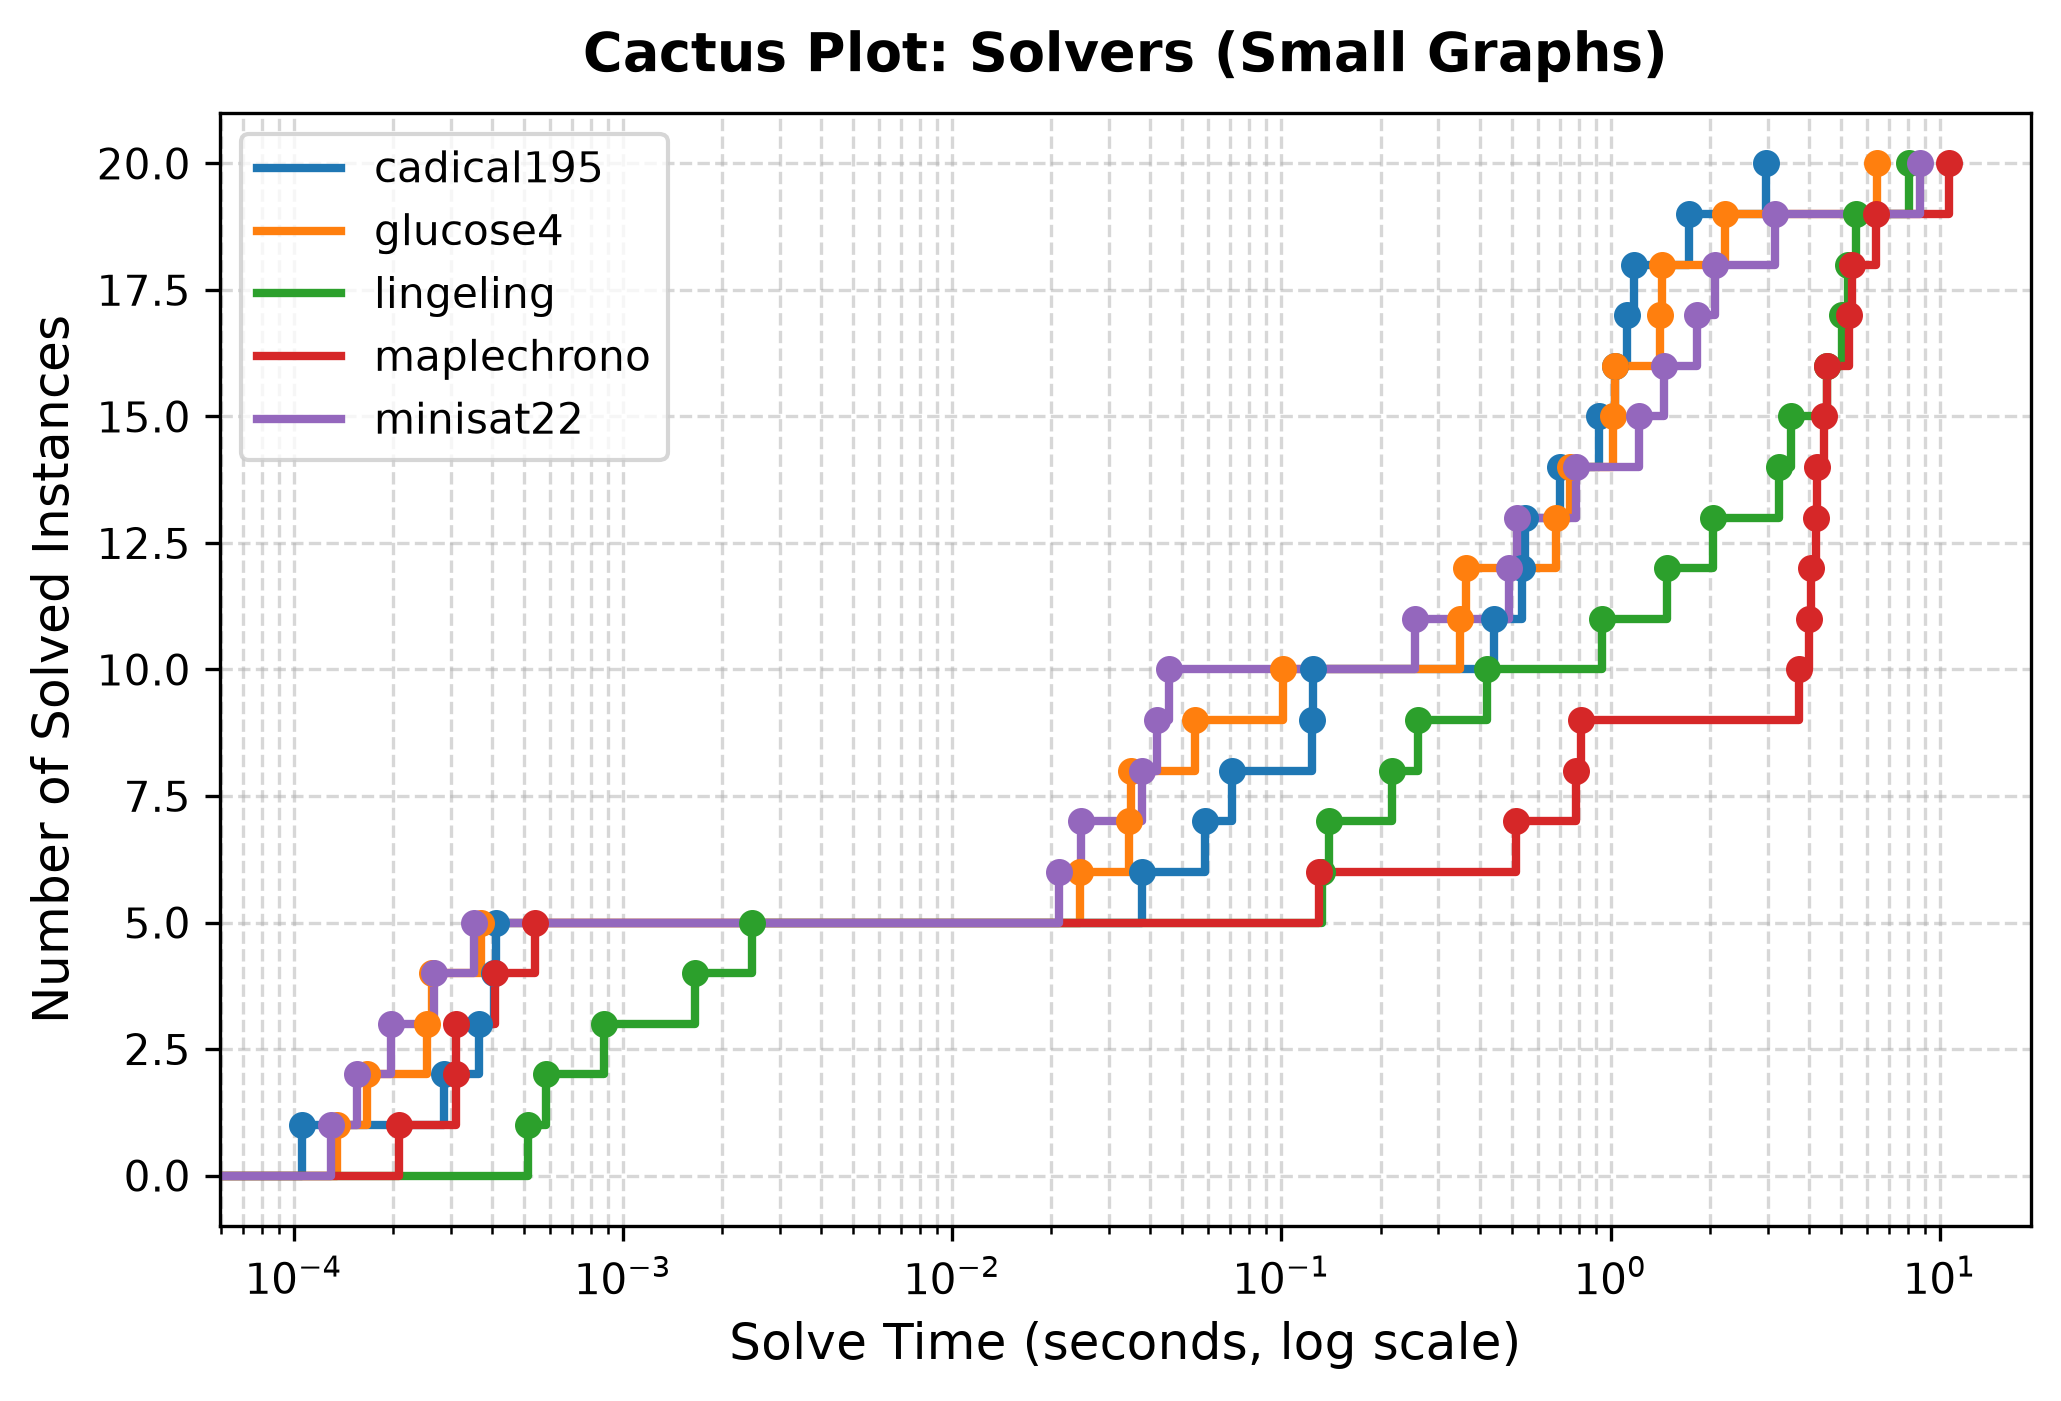
\includegraphics[width=0.48\textwidth]{figures/cactus_solvers_small}
\hfill
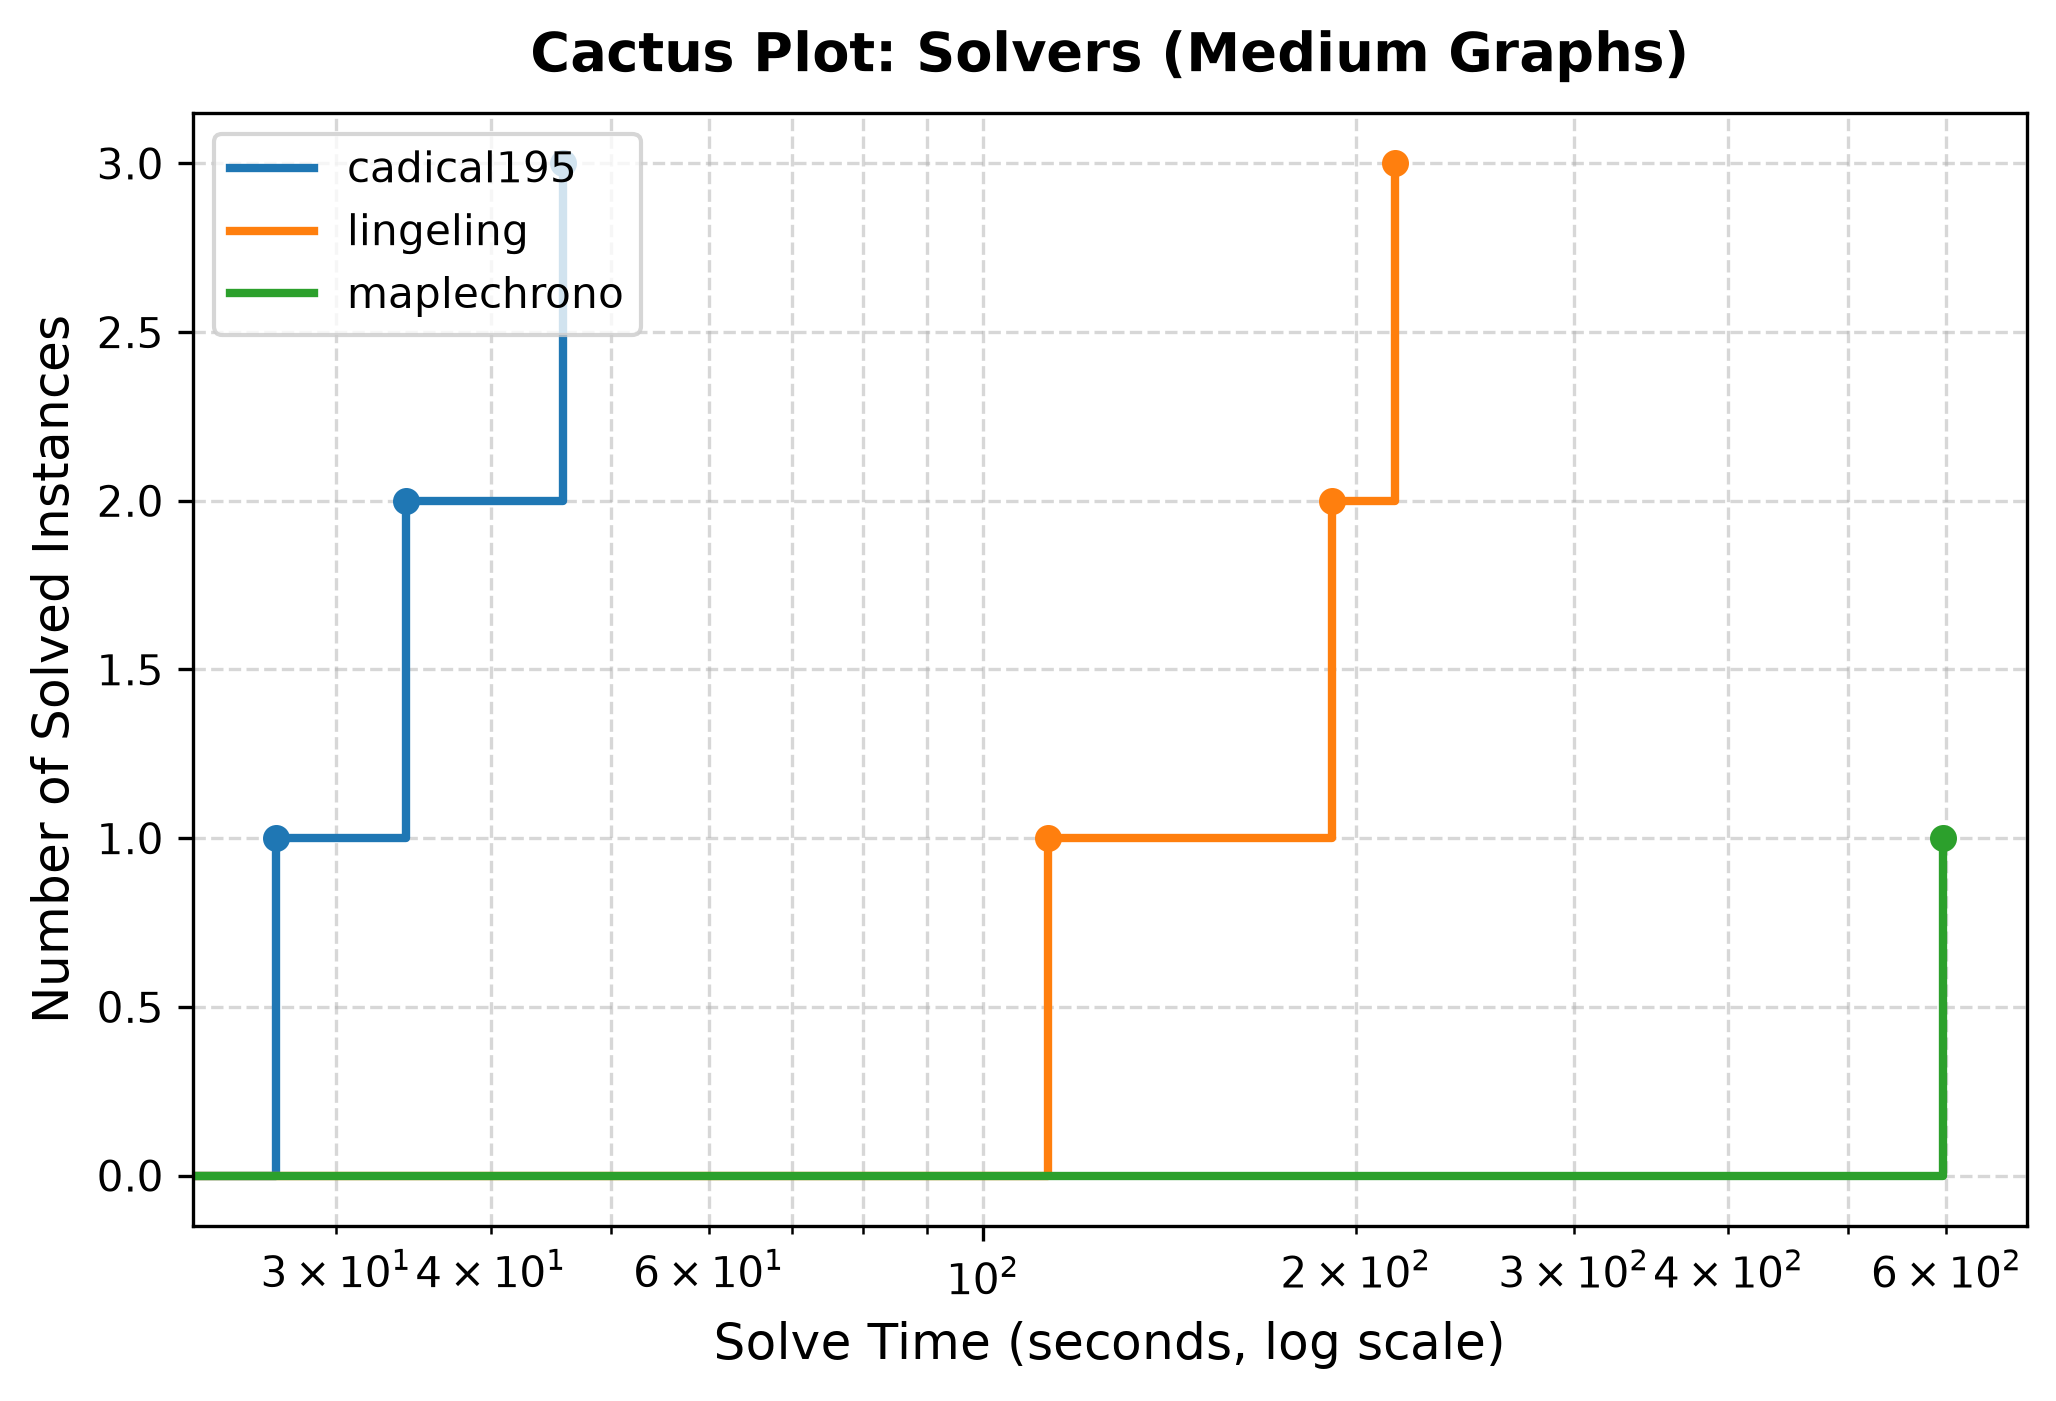
\includegraphics[width=0.48\textwidth]{figures/cactus_solvers_medium}
\caption{Cactus plots comparing SAT solver runtimes on small graphs (left) and medium graphs (right).}
\label{fig:cactus_solvers}
\end{figure}

\subsection{Method Comparison: SAT vs. CP-SAT vs. CPLEX}
Table~\ref{tab:table_methods} compares our best SAT configuration (CaDiCaL~195 with rotation, reflection, and RCM upper bound) against OR-Tools CP-SAT and IBM CPLEX across 7 small and medium instances.

% --- TABLE 3: METHODS COMPARISON ---
\begin{table}
\centering
\caption{Comparison of Methods: Best SAT vs. OR-Tools CP-SAT vs. IBM CPLEX}
\label{tab:table_methods}
\begin{tabular}{lrrrrr}
\toprule
Dataset & $N$ & $|E|$ & Best SAT & CP-SAT & CPLEX \\
\midrule
\texttt{14\_bus} & 14 & 20 & \textbf{0.0004} & 0.0328 & 0.4610 \\
\texttt{30\_bus} & 30 & 39 & \textbf{0.0547} & 0.2842 & SL \\
\texttt{494\_bus\_n40} & 40 & 52 & \textbf{0.7132} & 1.3461 & SL \\
\texttt{662\_bus\_n40} & 40 & 50 & 1.7629 & \textbf{0.5772} & SL \\
\texttt{494\_bus\_n60} & 60 & 76 & 34.1434 & \textbf{5.2765} & SL \\
\texttt{662\_bus\_n60} & 60 & 77 & 26.8385 & \textbf{5.5421} & SL \\
\texttt{662\_bus\_n80} & 80 & 105 & \textbf{45.7719} & 101.2120 & SL \\
\midrule
\textbf{Solved} & - & - & \textbf{7/7} & \textbf{7/7} & 1/7 \\
\textbf{Size Limit (SL)} & - & - & 0 & 0 & \textbf{6} \\
\textbf{Mean Time (s)} & - & - & \textbf{15.612} & 16.324 & - \\
\textbf{Speedup (geom) [5/7]} & - & - & 1.00$\times$ & \textbf{1.87$\times$} & - \\
\bottomrule
\multicolumn{6}{l}{\footnotesize SL: Exceeded Community Edition limit ($\le 1000$ variables/constraints). Speedup computed over instances $\ge 0.1\text{s}$.} \\
\end{tabular}
\end{table}

\paragraph{CPLEX MIP Baseline:} CPLEX solves only \texttt{14\_bus} ($N=14$, 0.461~s). For all instances with $N \ge 30$, CPLEX exceeds the 1000-variable Community Edition threshold and aborts with a Size Limit (SL) status. This illustrates the acute modeling overhead of MIP for non-linear cyclic distance metrics.

\paragraph{SAT vs. CP-SAT:} Both Best SAT and CP-SAT solve all 7 instances to global optimality. CP-SAT demonstrates fast filtering on the $N=60$ instances (\texttt{494\_bus\_n60}: 5.28~s vs. 34.14~s; \texttt{662\_bus\_n60}: 5.54~s vs. 26.84~s), leveraging integer domain propagation. However, as graph size scales to $N=80$ (\texttt{662\_bus\_n80}), SAT decisively outperforms CP-SAT (45.77~s vs. 101.21~s, a $2.21\times$ speedup for SAT). Across all 7 instances, SAT achieves a lower mean runtime (15.61~s vs. 16.32~s).

% --- TABLE 4: METHODS LARGE ---
\begin{table}
\centering
\footnotesize
\setlength{\tabcolsep}{4.5pt}
\caption{Comparison of Methods on Large Graphs ($N \ge 80$, Original Labels)}
\label{tab:table_methods_large}
\begin{tabular}{lrrrrrrrrr}
\toprule
Dataset & $N$ & $|E|$ & SAT Stat & SAT UB & SAT (s) & CP-SAT Stat & CP-SAT UB & $LB_{\text{comb}}$ & CP-SAT (s) \\
\midrule
\texttt{494\_bus\_n80} & 80 & 97 & \textbf{OPT} & 8 & 370.97 & \textbf{OPT} & 8 & 8 & 12.33 \\
\texttt{494\_bus\_n100} & 100 & 118 & \textbf{OPT} & 9 & 249.38 & \textbf{OPT} & 9 & 9 & 108.01 \\
\texttt{662\_bus\_n100} & 100 & 130 & \textbf{OPT} & 11 & \textbf{235.54} & TO & 12 & 5 & 600.01 \\
\texttt{494\_bus\_n150} & 150 & 175 & TO & 13 & 391.08 & TO & 20 & 5 & 600.01 \\
\texttt{662\_bus\_n150} & 150 & 190 & TO & 17 & 158.28 & TO & 20 & 5 & 600.01 \\
\texttt{494\_bus} & 494 & 586 & TO & 63 & 596.88 & TO & 54 & 5 & 600.01 \\
\texttt{662\_bus} & 662 & 906 & TO & 131 & 484.08 & TO & 147 & 5 & 600.02 \\
\bottomrule
\multicolumn{10}{l}{\footnotesize OPT: Proved optimal; TO: Timeout (600s). $LB_{\text{comb}} = \max(LB_{\text{degree}}, \text{cpsat\_solver\_lb})$. SAT (s) is accumulated solve time.} \\
\end{tabular}
\end{table}

\paragraph{Large Graph Scaling ($N \ge 80$):}
Table~\ref{tab:table_methods_large} evaluates large instances up to $N=662$. Remarkably, on \texttt{662\_bus\_n100} ($N=100, |E|=130$), Best SAT proves the global optimum ($\text{UB}^* = 11$) in 235.54~seconds, whereas CP-SAT times out at 600~seconds with an unproven bound of 12. For $N \ge 150$, both approaches time out at 600~seconds, yet SAT consistently yields competitive or tighter incumbent upper bounds during intermediate iterations (e.g., 13 vs. 20 on \texttt{494\_bus\_n150}, and 17 vs. 20 on \texttt{662\_bus\_n150}).

% --- TABLE: PER DATASET SUMMARY ---
\begin{table}
\centering
\caption{Comprehensive SAT Optimization Results Across All 16 Benchmark Graphs}
\label{tab:table_per_dataset}
\begin{tabular}{lrrrrrrrr}
\toprule
Dataset & $N$ & $|E|$ & Status & $\text{UB}^*$ & $LB_{\text{deg}}$ & Solve Time (s) & Wall Time (s) & Iterations \\
\midrule
\texttt{14\_bus} & 14 & 20 & OPTIMAL & 3 & 3 & 0.0004 & 0.65 & 3 \\
\texttt{30\_bus} & 30 & 39 & OPTIMAL & 4 & 2 & 0.0547 & 0.62 & 4 \\
\texttt{494\_bus\_n40} & 40 & 52 & OPTIMAL & 5 & 5 & 0.7132 & 1.29 & 11 \\
\texttt{662\_bus\_n40} & 40 & 50 & OPTIMAL & 7 & 5 & 1.7629 & 2.34 & 8 \\
\texttt{494\_bus\_n50} & 50 & 65 & OPTIMAL & 6 & 5 & 4.6657 & 5.35 & 11 \\
\texttt{662\_bus\_n50} & 50 & 64 & OPTIMAL & 8 & 5 & 1.1949 & 1.75 & 6 \\
\texttt{494\_bus\_n60} & 60 & 76 & OPTIMAL & 7 & 5 & 34.1434 & 34.79 & 10 \\
\texttt{662\_bus\_n60} & 60 & 77 & OPTIMAL & 9 & 5 & 26.8385 & 27.39 & 13 \\
\texttt{494\_bus\_n80} & 80 & 97 & OPTIMAL & 8 & 5 & 370.9714 & 371.57 & 9 \\
\texttt{662\_bus\_n80} & 80 & 105 & OPTIMAL & 10 & 5 & 45.7719 & 46.45 & 8 \\
\texttt{494\_bus\_n100} & 100 & 118 & OPTIMAL & 9 & 5 & 249.3777 & 250.15 & 13 \\
\texttt{662\_bus\_n100} & 100 & 130 & OPTIMAL & 11 & 5 & 235.5427 & 236.31 & 14 \\
\texttt{494\_bus\_n150} & 150 & 175 & TIMEOUT & 13 & 5 & 391.0825 & 600.48 & 18 \\
\texttt{662\_bus\_n150} & 150 & 190 & TIMEOUT & 17 & 5 & 158.2803 & 600.49 & 16 \\
\texttt{494\_bus} & 494 & 586 & TIMEOUT & 63 & 5 & 596.8806 & 600.52 & 6 \\
\texttt{662\_bus} & 662 & 906 & TIMEOUT & 131 & 5 & 484.0771 & 600.54 & 6 \\
\bottomrule
\multicolumn{9}{l}{\footnotesize Note: Solve Time is cumulative time across all SAT iterations. Wall Time includes Python process lifecycle and encoding.} \\
\end{tabular}
\end{table}

\subsection{Ablation Study}
To dissect the contribution of each algorithmic component, we evaluate five variants under identical solver settings (CaDiCaL~195):
\begin{itemize}
    \item \texttt{none}: Baseline without symmetry breaking and with trivial upper bound ($\lfloor N/2 \rfloor + 1$).
    \item \texttt{rotation}: With rotation symmetry breaking ($f(v_0) = 0$).
    \item \texttt{rot\_ref}: With both rotation and reflection symmetry breaking ($f(v_1) < f(v_{N-1})$).
    \item \texttt{heur\_ub}: With RCM initial upper bound alone.
    \item \texttt{all}: Combining rotation, reflection, and RCM upper bound.
\end{itemize}

% --- TABLE 5: ABLATION SMALL ---
\begin{table}
\centering
\caption{Ablation Study on Small Graphs ($N \le 40$, Mean over 5 Repetitions)}
\label{tab:table_ablation_small}
\begin{tabular}{lrrrrrrr}
\toprule
Dataset & $N$ & $|E|$ & \texttt{none} & \texttt{rotation} & \texttt{rot\_ref} & \texttt{heur\_ub} & \texttt{all} \\
\midrule
\texttt{14\_bus} & 14 & 20 & 0.0016 & 0.0003 & 0.0003 & 0.0032 & \textbf{0.0002} \\
\texttt{30\_bus} & 30 & 39 & 0.6624 & 0.1140 & 0.0537 & 0.6789 & \textbf{0.0527} \\
\texttt{494\_bus\_n40} & 40 & 52 & 2.2366 & \textbf{0.4966} & 1.0584 & 4.9084 & 0.7135 \\
\texttt{662\_bus\_n40} & 40 & 50 & 5.4982 & \textbf{0.2405} & 0.8778 & 9.8131 & 1.7468 \\
\midrule
\textbf{Solved} & - & - & 4/4 & 4/4 & 4/4 & 4/4 & 4/4 \\
\textbf{Mean Time (s)} & - & - & 2.102 & \textbf{0.213} & 0.499 & 3.853 & 0.638 \\
\textbf{Speedup (geom) [3/4]} & - & - & 1.00$\times$ & \textbf{8.42$\times$} & 5.47$\times$ & 0.63$\times$ & 4.99$\times$ \\
\bottomrule
\multicolumn{8}{l}{\footnotesize Speedup computed over instances with baseline runtime $\ge 0.1\text{s}$.} \\
\end{tabular}
\end{table}

% --- TABLE 6: ABLATION MEDIUM ---
\begin{table}
\centering
\caption{Ablation Study on Medium Boundary Graph (\texttt{662\_bus\_n60})}
\label{tab:table_ablation_medium}
\begin{tabular}{lrrrrrrr}
\toprule
Dataset & $N$ & $|E|$ & \texttt{none} & \texttt{rotation} & \texttt{rot\_ref} & \texttt{heur\_ub} & \texttt{all} \\
\midrule
\texttt{662\_bus\_n60} & 60 & 77 & 279.44 & 46.48 & \textbf{12.27} & 74.46 & 26.97 \\
\midrule
\textbf{Solved} & - & - & 1/1 & 1/1 & 1/1 & 1/1 & 1/1 \\
\textbf{Speedup (geom) [1/1]} & - & - & 1.00$\times$ & 6.01$\times$ & \textbf{22.77$\times$} & 3.75$\times$ & 10.36$\times$ \\
\bottomrule
\end{tabular}
\end{table}

\paragraph{Impact of Rotation Symmetry Breaking:}
As shown in Table~\ref{tab:table_ablation_small}, adding rotation symmetry breaking alone (\texttt{rotation}) provides an overwhelming performance improvement, reducing mean solve time from 2.102~s to 0.213~s on small graphs (an $8.42\times$ geometric speedup). On the medium instance \texttt{662\_bus\_n60} (Table~\ref{tab:table_ablation_medium}), rotation symmetry breaking reduces runtime from 279.44~s to 46.48~s ($6.01\times$ speedup). By eliminating $N$ circularly shifted permutations, rotation symmetry breaking eliminates entire subtrees of isomorphic assignments.

\paragraph{Impact of Reflection Symmetry Breaking:}
When reflection symmetry breaking is added on top of rotation (\texttt{rot\_ref}), the effect depends on instance size:
\begin{itemize}
    \item On small graphs ($N \le 40$), the addition of $N$ ternary clauses slightly increases clause density without substantially reducing search depth, resulting in a moderate speedup ($5.47\times$ vs. $8.42\times$ for rotation alone).
    \item On medium graphs (\texttt{662\_bus\_n60}), reflection symmetry breaking delivers a spectacular performance boost: solve time plummets from 46.48~s down to 12.27~s, delivering a combined \textbf{22.77$\times$ speedup} over \texttt{none}.
\end{itemize}

\paragraph{Impact of Initial Heuristic Upper Bound:}
Using the RCM heuristic alone (\texttt{heur\_ub}) without symmetry breaking results in a slowdown on small graphs (0.63$\times$ speedup, mean time 3.85~s vs. 2.10~s). This occurs because starting from a tighter bound forces the solver immediately into hard, highly-constrained subproblems without eliminating symmetric UNSAT branches. However, when combined with symmetry breaking (\texttt{all}), the RCM bound prunes intermediate SAT iterations while symmetry breaking keeps the final UNSAT proof manageable.

% --- TABLE 7: ABLATION FAMILY ---
\begin{table}
\centering
\caption{Ablation Study Across Graph Families Under Random Vertex Relabeling (30 Pairs)}
\label{tab:table_ablation_family}
\begin{tabular}{llrrrr}
\toprule
Comparison Group & Variant & Median Time Ratio & IQR [25\%, 75\%] & [Min, Max] & Faster Pairs \\
\midrule
Variant vs. \texttt{none} & \texttt{rotation} & 0.4506 & [0.2992, 0.7606] & [0.1085, 1.2073] & \textbf{28/30} \\
Variant vs. \texttt{none} & \texttt{rot\_ref} & 0.5189 & [0.2866, 0.9944] & [0.1867, 1.6154] & 22/30 \\
Variant vs. \texttt{none} & \texttt{heur\_ub} & 0.8544 & [0.6120, 1.0007] & [0.3879, 2.3016] & 22/30 \\
Variant vs. \texttt{none} & \texttt{all} & \textbf{0.4043} & [0.2792, 0.6705] & [0.1094, 1.1330] & \textbf{27/30} \\
\midrule
\texttt{rot\_ref} vs. \texttt{rotation} & \texttt{rot\_ref} & 1.1360 & [0.9261, 1.3825] & [0.5898, 1.8817] & 12/30 \\
\texttt{all} vs. \texttt{rot\_ref} & \texttt{all} & 0.8037 & [0.5404, 1.2279] & [0.1116, 1.8718] & 21/30 \\
\texttt{all} vs. \texttt{rotation} & \texttt{all} & 0.8785 & [0.6430, 1.2980] & [0.2100, 2.1826] & 19/30 \\
\bottomrule
\multicolumn{6}{l}{\footnotesize Note: Evaluated on \texttt{494\_bus\_n40} (10 seeds), \texttt{662\_bus\_n40} (10 seeds), \texttt{494\_bus\_n50} (5 seeds), \texttt{662\_bus\_n50} (5 seeds).} \\
\end{tabular}
\end{table}

\paragraph{Statistical Evaluation on Relabeled Graph Families:}
To avoid bias from arbitrary vertex orderings, Table~\ref{tab:table_ablation_family} reports pairwise runtime ratios across 30 randomized graph instances (10 seeds on \texttt{n40} and 5 seeds on \texttt{n50}). The combined configuration \texttt{all} achieves a median runtime ratio of \textbf{0.4043} relative to \texttt{none} (over a $59\%$ reduction in median runtime) and is faster in \textbf{27 out of 30 pairs}. Rotation alone is faster in \textbf{28 out of 30 pairs} (median ratio 0.4506).

\begin{figure}
\centering
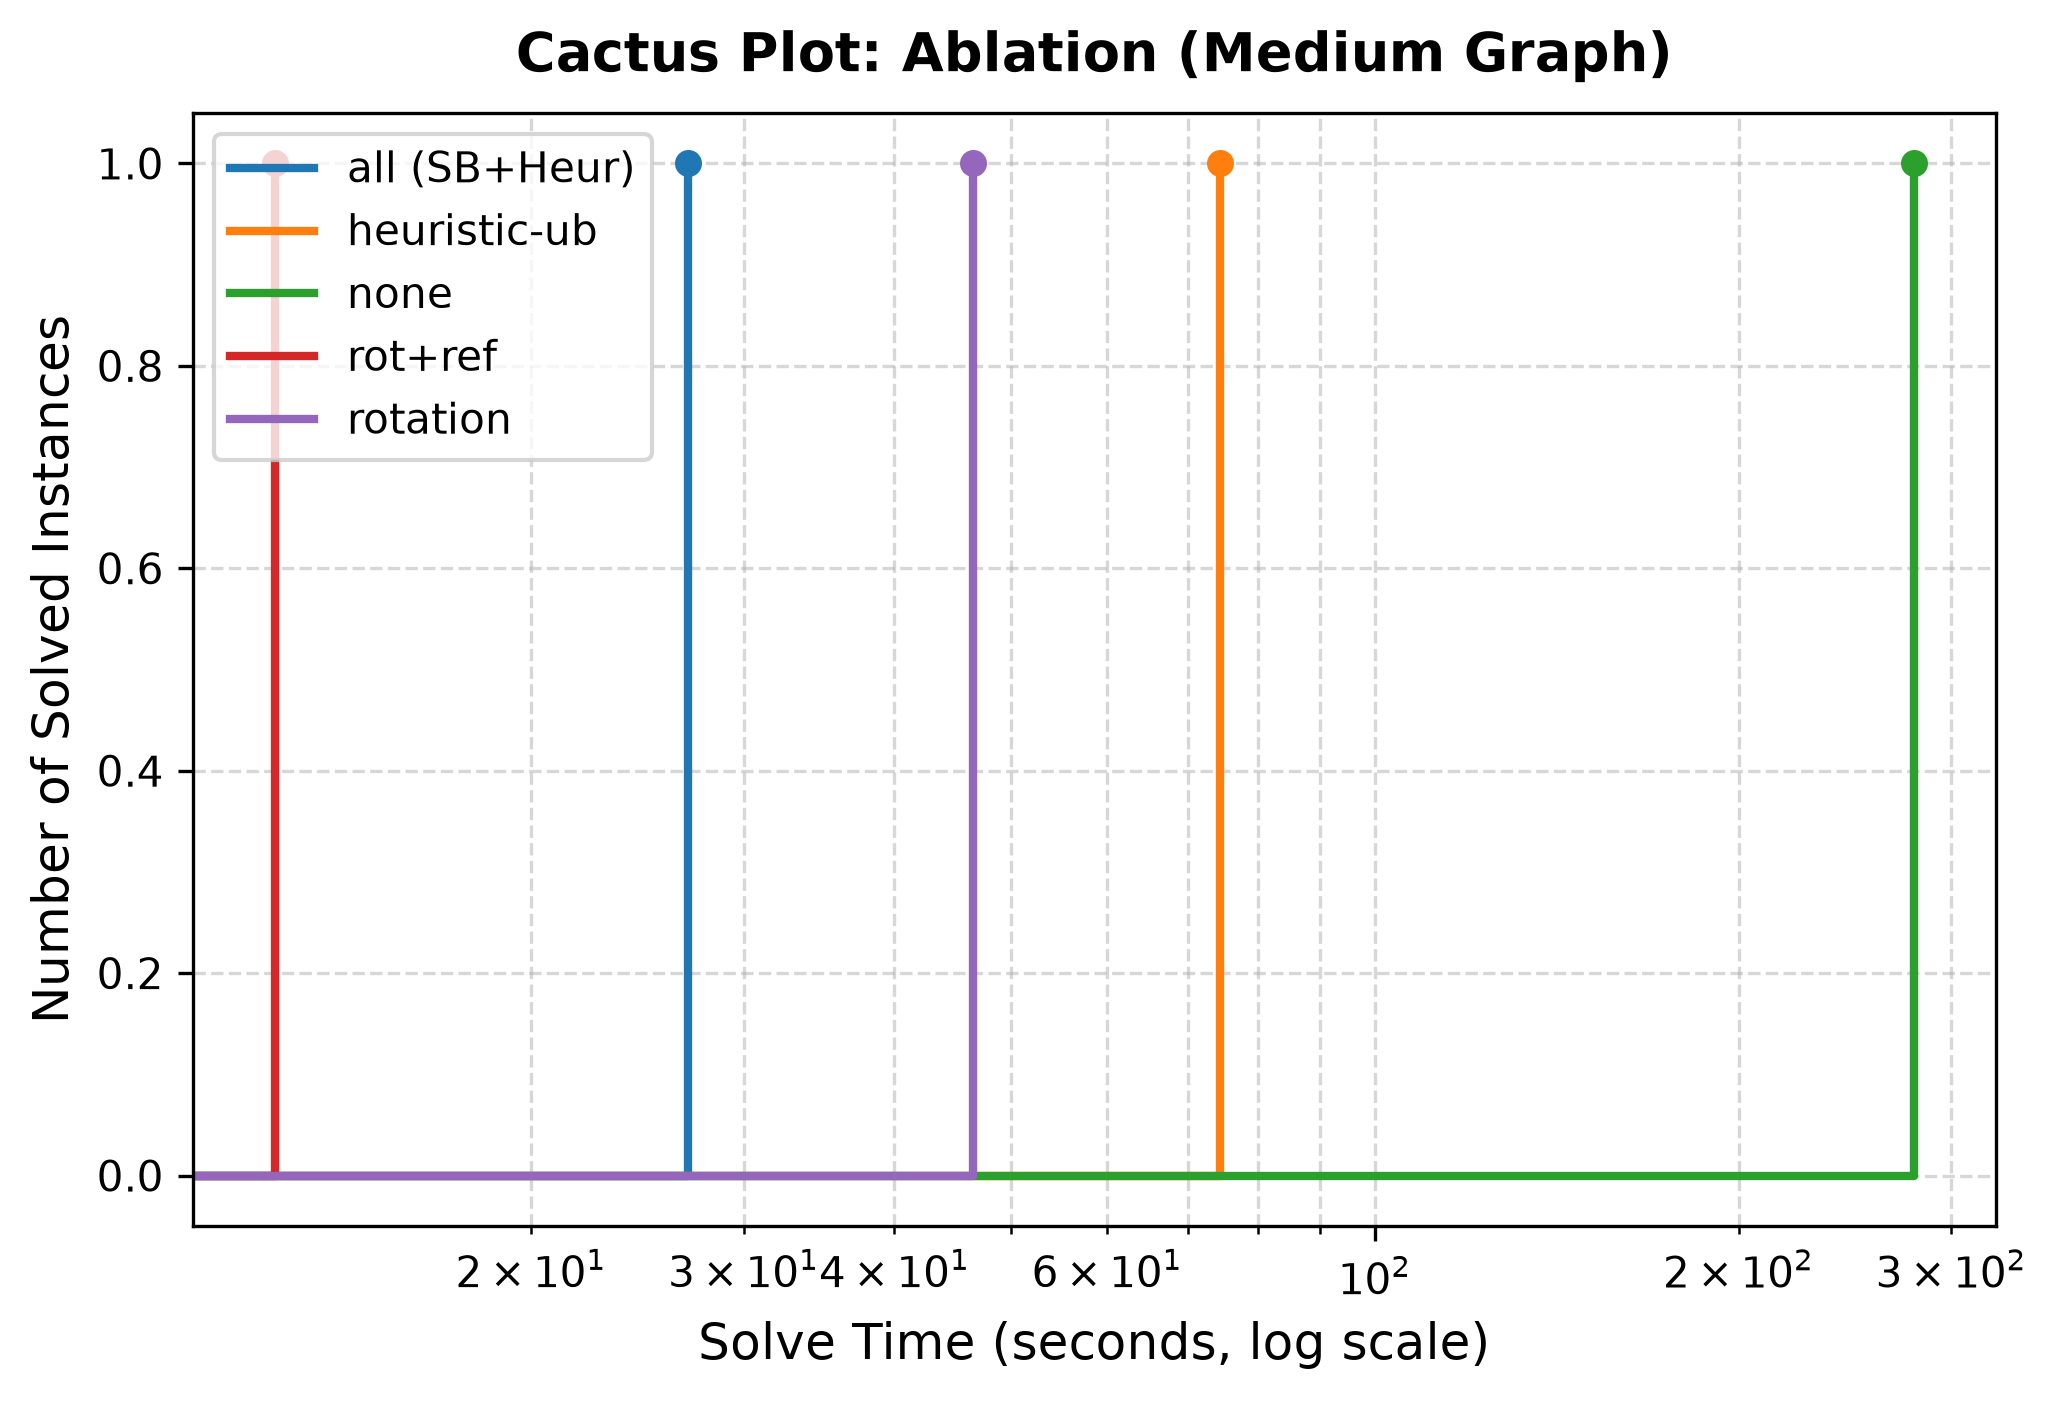
\includegraphics[width=0.48\textwidth]{figures/cactus_ablation_medium}
\hfill
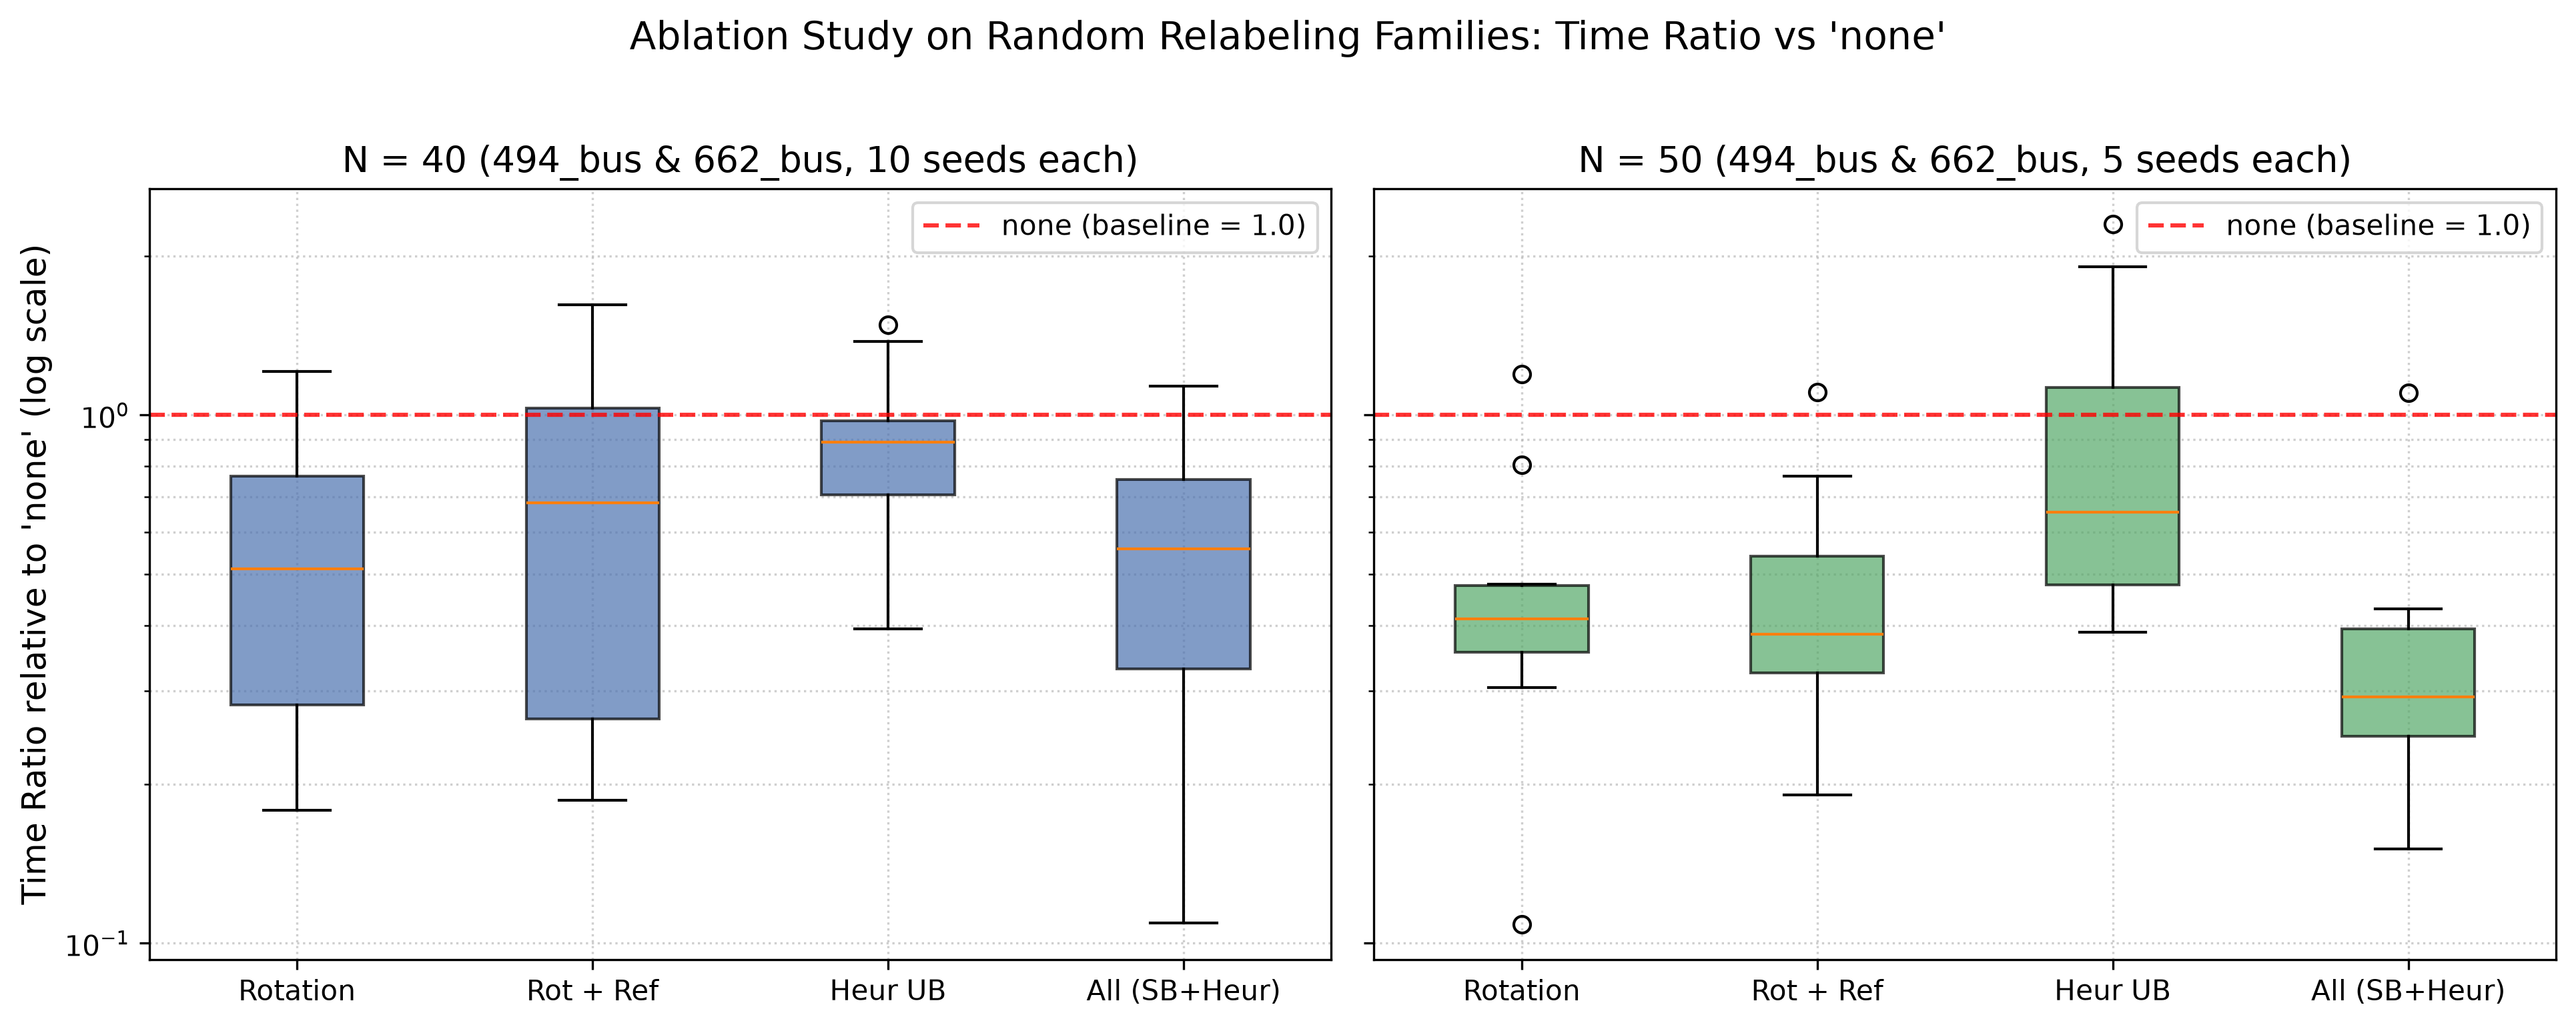
\includegraphics[width=0.48\textwidth]{figures/boxplot_ablation_family}
\caption{Ablation performance: Medium graph cactus plot (left) and runtime ratio boxplots across 30 relabeled graph family instances (right).}
\label{fig:ablation_plots}
\end{figure}

\subsection{Phase Analysis: SAT Feasibility vs. UNSAT Optimality Proof}
To understand why symmetry breaking is so effective, we separate the execution time into two phases:
\begin{enumerate}
    \item \textbf{Previous Iterations Time ($T_{\text{prev}}$)}: The cumulative time spent in satisfiable iterations finding tighter incumbent layouts.
    \item \textbf{Last Iteration Time ($T_{\text{last}}$)}: The time spent in the final unsatisfiable call proving that no layout with bandwidth $\le \text{UB}^* - 1$ exists.
\end{enumerate}

% --- TABLE 8: ABLATION PHASES ---
\begin{table}
\centering
\caption{Phase Decomposition: Median Times and Ratio of Final UNSAT Step}
\label{tab:table_ablation_phases}
\begin{tabular}{rlrrr}
\toprule
Graph Size ($N$) & Variant & Median $T_{\text{last}}$ (s) & Median $T_{\text{prev}}$ (s) & UNSAT Fraction ($T_{\text{last}} / T_{\text{total}}$) \\
\midrule
40 & \texttt{none} & 1.1557 & 0.6861 & 67.21\% \\
40 & \texttt{rotation} & 0.2552 & 0.5823 & 34.24\% \\
40 & \texttt{rot\_ref} & 0.3789 & 0.4786 & 46.33\% \\
40 & \texttt{heur\_ub} & 0.7635 & 0.6022 & 61.07\% \\
40 & \texttt{all} & \textbf{0.2099} & 0.5307 & \textbf{25.41\%} \\
\midrule
50 & \texttt{none} & 14.6611 & 1.1817 & \textbf{90.82\%} \\
50 & \texttt{rotation} & 4.5502 & 1.4048 & 72.15\% \\
50 & \texttt{rot\_ref} & 3.4413 & 2.1841 & 64.82\% \\
50 & \texttt{heur\_ub} & 6.8488 & 1.6089 & 78.50\% \\
50 & \texttt{all} & \textbf{2.3708} & 0.9201 & \textbf{76.55\%} \\
\bottomrule
\end{tabular}
\end{table}

Table~\ref{tab:table_ablation_phases} presents the results. On unaugmented search (\texttt{none}), proving UNSAT accounts for \textbf{67.21\%} of runtime at $N=40$ and surges to \textbf{90.82\%} at $N=50$ (14.66~s out of 15.84~s). Because an UNSAT proof requires refuting the entire search space, exploring symmetric branches exponentially inflates refutation size. Rotation and reflection symmetry breaking shrink the refutation proof directly: for $N=50$, \texttt{all} slashes the final UNSAT time from 14.66~s down to \textbf{2.37~s} (a $6.19\times$ reduction in proof time).

\subsection{Discussion and Limitations}
Our empirical findings reveal clear trade-offs:
\begin{enumerate}
    \item \textbf{Symmetry Breaking Overhead vs. Pruning}: On very small graphs ($N \le 30$), symmetry breaking overhead is negligible, but so is search space size. On medium and hard graphs ($N \ge 60$), symmetry breaking provides orders-of-magnitude acceleration.
    \item \textbf{Scalability Ceiling}: Beyond $N = 100$, CNF clause generation scales as $\mathcal{O}(|E| \cdot N + N^2)$. For $N = 494$, the formula requires roughly 500,000 variables and millions of clauses, leading to memory pressure and timeout during incremental solving. Future work should investigate pseudo-Boolean encodings or lazy clause generation to mitigate clausal expansion.
\end{enumerate}

% =========================================================================
\section{Conclusion}
% =========================================================================

In this work, we presented an exact SAT-based framework for the Cyclic Bandwidth Minimization Problem (CBMP). By integrating Order Encoding for circular distance bounds, Commander Encoding for bijective permutation constraints, and mathematically sound rotation and reflection symmetry breaking, our approach prunes the $2N$-fold dihedral symmetry inherent to circular layouts.

We evaluated the framework on 16 benchmark graphs against state-of-the-art SAT, CP, and MIP solvers. Our findings establish that:
\begin{enumerate}
    \item CaDiCaL~195 is the top-performing SAT engine for CBMP, solving medium and large instances where Glucose~4, MiniSat~2.2, and MapleChrono time out.
    \item Dual symmetry breaking achieves up to a $22.77\times$ speedup on medium boundary graphs and reduces median solve time across randomized graph families by more than $59\%$.
    \item The final UNSAT proof dominates up to $90\%$ of overall runtime, and symmetry breaking provides its greatest acceleration by directly shrinking this refutation proof.
    \item Best SAT scales beyond commercial MIP and outperforms CP-SAT on challenging instances (e.g., proving optimality on \texttt{662\_bus\_n100} where CP-SAT times out).
\end{enumerate}
Future work will focus on integrating graph decomposition techniques and exploring lazy clause generation architectures to extend exact CBMP solving to graphs with several hundreds of vertices.

% =========================================================================
% REFERENCES
% =========================================================================
\begin{thebibliography}{15}

\bibitem{diaz2002survey}
J.~D\'{\i}az, J.~Petit, and M.~Serna, ``A survey of graph layout problems,'' \emph{ACM Computing Surveys}, vol.~34, no.~3, pp.~313--356, 2002.

\bibitem{leung1984cyclic}
J.~Y.-T. Leung, O.~Vornberger, and J.~D. Witthoff, ``On some variants of the bandwidth minimization problem,'' \emph{SIAM Journal on Computing}, vol.~13, no.~3, pp.~650--667, 1984.

\bibitem{kahng2011vlsilayout}
A.~B. Kahng, J.~Lienig, I.~L. Markov, and J.~Hu, \emph{VLSI Physical Design: From Graph Partitioning to Timing Closure}, Springer Science \& Business Media, 2011.

\bibitem{cuthill1969rcm}
E.~Cuthill and J.~McKee, ``Reducing the bandwidth of sparse symmetric matrices,'' in \emph{Proceedings of the 1969 24th National Conference of the ACM}, pp.~157--172, 1969.

\bibitem{biere2021handbook}
A.~Biere, M.~Heule, H.~van Maaren, and T.~Walsh, Eds., \emph{Handbook of Satisfiability}, 2nd~ed., IOS Press, 2021.

\bibitem{tamura2009order}
N.~Tamura, A.~Taga, S.~Kitagawa, and M.~Banbara, ``Compiling finite domain constraints to SAT with order encoding,'' \emph{Modeling and Computation in Environmental Sciences}, vol.~19, no.~4, pp.~257--264, 2009.

\bibitem{klieber2007efficient}
W.~Klieber and G.~Kwon, ``Efficient CNF encoding for selecting 1 from $n$ objects,'' in \emph{Fourth Workshop on Constraints in Formal Verification (CFV)}, 2007.

\bibitem{biere2020cadical}
A.~Biere, K.~Fazekas, M.~Fleury, and M.~Heisinger, ``CaDiCaL, Kissat, Paracooba, Plingeling and Treengeling entering the SAT Competition 2020,'' in \emph{Proceedings of SAT Competition 2020 -- Solver and Benchmark Descriptions}, Department of Computer Science Report Series B, vol.~B-2020-1, pp.~51--53, University of Helsinki, 2020.

\bibitem{audemard2009glucose}
G.~Audemard and L.~Simon, ``Predicting learnt clauses quality in modern SAT solvers,'' in \emph{Proceedings of the 21st International Joint Conference on Artificial Intelligence (IJCAI 2009)}, pp.~399--404, 2009.

\bibitem{een2003minisat}
N.~E\'en and N.~S\"orensson, ``An extensible SAT-solver,'' in \emph{Theory and Applications of Satisfiability Testing (SAT 2003)}, Lecture Notes in Computer Science, vol.~2919, pp.~502--518, Springer, 2004.

\bibitem{liang2016maple}
J.~H. Liang, V.~Ganesh, P.~Poupart, and K.~Czarnecki, ``Learning rate based branching heuristic for SAT solvers,'' in \emph{Theory and Applications of Satisfiability Testing (SAT 2016)}, Lecture Notes in Computer Science, vol.~9710, pp.~123--140, Springer, 2016.

\bibitem{ignatiev2018pysat}
A.~Ignatiev, A.~Morgado, and J.~Marques-Silva, ``PySAT: A Python toolkit for prototyping with SAT oracles,'' in \emph{International Conference on Theory and Applications of Satisfiability Testing (SAT)}, pp.~428--437, 2018.

\bibitem{perron2021ortools}
L.~Perron and V.~Furnon, ``OR-Tools,'' Google, version 9.15, \url{https://developers.google.com/optimization}.

\bibitem{cplex2026}
IBM Corp., ``IBM ILOG CPLEX Optimization Studio CPLEX User's Manual,'' version 22.2.0.0, \url{https://www.ibm.com/docs/en/icos}.

\end{thebibliography}

\end{document}
